% Chapter 1
\section{The current state of online learning}
\phantomsection
In recent years, online learning has seen a massive boom: thousands of people
enroll each year in online classes, some of these being complementary to the
traditional courses, some being only available online. The second option has
spawn a whole new branch of e-learning, called Massive Open Online Courses, or
MOOC.

\subsection{How does education benefit from going online}
Bringing education online takes advantages of connectivity similar to those of
social networks, reaching and engaging a very wide audience.  One of the major
appeal of the e-learning through MOOC's, is that the course can be taken by an
large number of students. Also, when the privacy and anonymity is a concern,
online courses provides obvious advantages: discrimination based on age, social status, or other
criteria is if not impossible, easily avoided. Online courses also give
students flexibility in their learning schedule, a highly customized timetable,
and provides them with high quality courses, that otherwise would be impossible
to attend, due to geographical location or financial reasons.
% leveling the playing field
MOOC education is also leveling the playing field: the third world student has
nothing else, and nowhere else to go, as vast amount of specialized knowledge
might not be available in that specific country. MOOC provide access for the
millions around the world who have no access to quality education.

\subsubsection{Economic advantage}
The economic advantage for education going
online can't be underestimated: Ernst \& Young cut training costs 35 percent
while improving consistency and scalability. They condensed about 2,900 hours of
classroom training into 700 hours of web-based learning, 200 hours of distance
learning and 500 hours of classroom instruction, a cut of 52
percent \citep{organisationalbenefits}.

\begin{figure}[!ht]
\centering
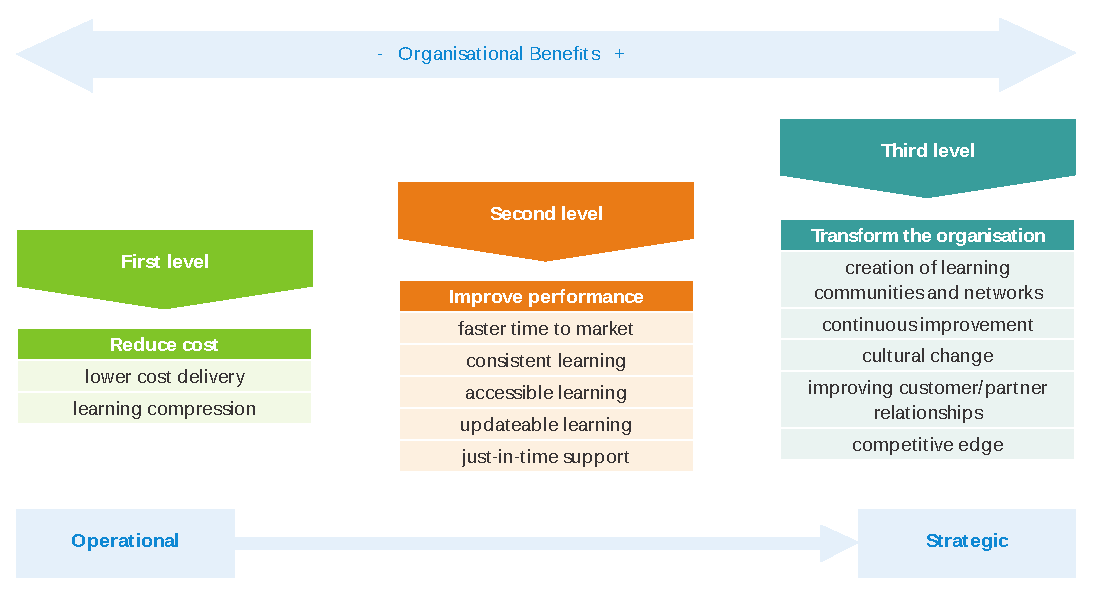
\includegraphics{organisational_benefits}
\caption{Organisational benefits of e-learning}
\label{fig:Organisational_benefits}
\end{figure}

\subsubsection{Speed of learning}
In addition to lower delivery costs there is a
strong argument that e-learning is more cost-effective because there is a
reduction in training time known as learning compression. This effect can speed
up the pace at which new employees get the necessary calification. This is
because the single largest cost of training in organizations is the cost of
staff attending the training course, rather than the direct delivery costs in
terms of trainers, course materials, travel and accommodation. E-learning can
deliver benefits by reducing the time it takes to train people because:
\begin{enumerate}
    \item[--] Learners can go at their own pace, not at the pace of the slowest member of a group, or someone gets left behind;
    \item[--] Time in classrooms can be spent on questions / topics introduced by other delegates that are irrelevant to the needs of the individual learner;
    \item[--] There is less time spent on social interaction;
    \item[--] It takes less time to start and wind up a learning session;
    \item[--] There is less travel time to and from a training event, or commuting to school;
    \item[--] Learners learn what they need to learn, they can skip elements of a program they don’t need.
\end{enumerate}
These factors can add up to an average compression (saving of learning time) of
35-45 percent when a course is taken out of the classroom and delivered in an
electronic format \citep{brandonhall}.

\subsubsection{Environmental issues}
Taking classes online can help the environment, by reducing waste and $ CO_{2} $.  The
Open University study \citep{openuniversity} examined in detail energy costs associated with classroom
learning in terms of $ CO_{2} $ emissions, and compared these to the costs of learning
via a computer. Computers are no environmental clean: They burn energy at least
0.125 kwh for a desktop PC, and can contain toxic materials such as lead,
cadmium, and PCB’s that pose serious health and environmental hazards. Despite
this, the $ CO_{2} $ emission levels associated with computer use were significantly
less than those associated with more conventional instructional delivery
methods, and much of the studying was done from home using computers that
students already owned, meaning that it would not change the balance in any way.

By taking lessons online, one can also save trees by saving paper. Many
e-learning courses are entirely self-contained, presenting all learning content
online, or providing alternatives to paper-based forms of communication through
such tools as email, PDF manuals, synchronous classrooms, and other web-based
tools, and there's no need to print out materials at all.

\subsubsection{Non-discrimitory environment}
The MOOC is open and invitational. No one who wishes to participate is excluded;
people negotiate the extent and nature of their participation according to their
individual needs and wishes, regardless of whether those needs are defined, for
example, by personal interest or workplace requirements. From a theoretical
perspective, this creates a very broad form of “legitimate peripheral
participation” \citep{wegner} which allows individuals to be drawn into the
community of practice at whatever rate is comfortable. From a pragmatic
perspective, this framework provides access to large numbers of people who
might otherwise be excluded for reasons ranging from time, to geographic
location, to formal prerequisites, to financial hardship \citep{wegner}.

If a course is well prepared, little to no guidance is necessary from the
teacher, and the knowledge can passed on for extended periods of time. With the
advances in storage technology, online courses can be kept basically forever, at
a low cost of storage, and basically zero cost for duplication.
% 2 pages

\subsection{The advent of MOOC}
% history, university of reddit, infographics
Before hitting the online realm, distance learning appeared in the form of
correspondence courses, broadcast courses and early forms of
e-learning \citep{history_of_instr_tech}. Over 4 million Americans
- far more than attended traditional colleges - were enrolled in correspondence
courses by the 1920s, covering hundreds of practical job-oriented topics. Their
completion rate was under 3\% \citep{pursuit_of_knowledge}.

Broadcast radio was new in the 1920s and with programs that were free to
audiences of any size \citep{listening_in}. By 1922, New York University operated its own radio
station, with plans to broadcast practically all its courses. Other schools
followed, including Columbia, Harvard, Kansas State, Ohio State, Purdue,
Wisconsin, Utah and many others. Students read textbooks and listened to
broadcast lectures, while mailing in answers to tests. Journalist Bruce Bliven
asked: "Is radio to become a chief arm of education? Will the classroom be
abolished and the child of the future be stuffed with facts as he sits at home
or even as he walks about the streets with his portable receiving-set in his
pocket?". Completion rates were very low, cheating was hard to detect, and
there was no way to collect tuition. By the 1940s radio courses had virtually
disappeared in the United States \citep{before_mooc}. The Australian School of the Air used
two-way shortwave radio starting in 1951 to teach students in classrooms in
remote locations, with students able to ask questions of the live instructor.

\subsubsection{The early approaches}
The first MOOCs emerged from the open educational resources (OER) movement. The
term MOOC was coined in 2008 by Dave Cormier of the University of Prince Edward
Island and Senior Research Fellow Bryan Alexander of the National Institute for
Technology in Liberal Education in response to a course called Connectivism and
Connective Knowledge (also known as CCK08). CCK08, which was led by George
Siemens of Athabasca University and Stephen Downes of the National Research
Council, consisted of 25 tuition-paying students in Extended Education at the
University of Manitoba, as well as over 2200 online students from the general
public who paid nothing. All course content was available through RSS feeds
and online students could participate through collaborative tools, including
blog posts, threaded discussions in Moodle and Second Life meetings \citep{cck08}.
Stephen Downes considers these so-called cMOOCs to be more "creative and
dynamic" than the current xMOOCs, which he believes "resemble television shows
or digital textbooks." \citep{courses_lack_of_creativity}

Galway based online education provider ALISON is often cited in industry
literature as the first MOOC, pioneering the systematic aggregation of online
interactive learning resources made available worldwide with a freemium
model. Its stated objective is to enable people to gain basic
education and workplace skills.Contrary to other MOOC providers with
close links to American third level institutions such as MIT and Stanford
University, the majority of ALISON's learners are located in the developing
world with the fastest growing number of users in India. It records 1.2
million unique visitors per month with 250,000 graduates of its 500+ courses as
of January 2013. In February 2014, ALISON registered its 3 millionth user.

%America
\subsubsection{MOOC in North America}
Several well-financed American providers emerged, associated with top
universities, including Udacity, Coursera, edX.
In the fall of 2011 Stanford University launched three courses. The first of
those courses was Introduction Into AI, launched by Sebastian Thrun and Peter
Norvig. Enrollment quickly reached 160,000 students. The announcement was
followed within weeks by the launch of two more MOOCs, by Andrew Ng and Jennifer
Widom. Following the publicity and high enrollment numbers of these courses,
Thrun started a company he named Udacity and Daphne Koller and Andrew Ng
launched Coursera. Coursera subsequently announced university partnerships with
University of Pennsylvania, Princeton University, Stanford University and The
University of Michigan.

Concerned about the commercialization of online education, MIT created the
not-for-profit MITx. The inaugural course, 6.002x, launched in March 2012.
Harvard joined the group, renamed edX, that spring, and University of
California, Berkeley joined in the summer. The initiative then added the
University of Texas System, Wellesley College and Georgetown University.

In November 2012, the University of Miami launched its first high school MOOC as
part of Global Academy, its online high school. The course became available for
high school students preparing for the SAT Subject Test in biology \citep{history_of_a_revolution}.

In January 2013, Udacity launched its first MOOCs-for-credit, in collaboration
with San Jose State University. In May 2013 the company announced the first
entirely MOOC-based Master's Degree, a collaboration between Udacity, AT\&T and
the Georgia Institute of Technology, costing \$7,000, a fraction of its normal
tuition.

In March 2013, Coursolve piloted a crowdsourced business strategy course for 100
organizations with the University of Virginia. A data science MOOC began in
May 2013.

In May 2013 Coursera announced free e-books for some courses in partnership with
Chegg, an online textbook-rental company. Students would use Chegg's e-reader,
which limits copying and printing and could use the book only while enrolled in
the class. In June 2013, the University of North Carolina at Chapel Hill
launched Skynet University, which offers MOOCs on introductory astronomy.
Participants gain access to the university's global network of robotic
telescopes, including those in the Chilean Andes and Australia. It incorporates
YouTube, Facebook and Twitter.

In September 2013, edX announced a partnership with Google to develop Open edX,
an open source platform and its MOOC.org, a site for non-xConsortium groups to
build and host courses. Google will work on the core platform development with
edX partners. In addition, Google and edX will collaborate on research into how
students learn and how technology can transform learning and teaching. MOOC.org
will adopt Google's infrastructure.

EdX currently offers 94 courses from 29 institutions around the world (as of
November 2013). During its first 13 months of operation (ending March 2013),
Coursera offered about 325 courses, with 30\% in the sciences, 28\% in arts and
humanities, 23\% in information technology, 13\% in business and 6\% in
mathematics. Udacity offered 26 courses. Udacity's CS101, with an enrollment
of over 300,000 students, was the largest MOOC to date.

% Europe
\subsubsection{MOOC in Europe}
Iversity is a MOOC provider in Germany. With over 82,000 students (Nov 2013)
iversity's "The Future of Storytelling" is Europe's largest MOOC to date.
OpenupEd is a supranational platform, founded with support of the European
Union (EU).

In Ireland ALISON provides free online certificate/diploma courses to two 2
million learners worldwide. ALISON was shortlisted in June 2013 by
London–based education technology company Edxus Group and specialist media and
advisory firm IBIS Capital, as one of the ``top 20 e-learning companies in
Europe' as judged by an expert panel.

In March 2013, a young entrepreneur Volkan Karabacak has started UniversitePlus
online courses system in Turkey to serve the region in Turkish, Russian, Arabic,
and other languages used in EurAsia. It is growing so fast by getting support
from higher education institutions from Turkey, Europe, and United States.

In October 2013, the French government announced the creation of France
Universite Numerique (FUN), a French public alternative to existing solutions.
French business schools have begun launching their own MOOCs, the first being
supervised by Alberto Alemanno.
% 3 pages
\subsection{Advantages of MOOC}

MOOC's have an economic edge over traditional education: not only it is cheaper
to train students online, but it can provide a stream o revenue for
universities: Coursera for example, is experimenting with a freemium model: the
content is given away for free, sometimes even Freely licensed, but the
certification process involves a fee.

Coursera, Udemy, EdX, Udacity are also considering several other business models:
\begin{enumerate}[topsep=5pt, partopsep=0pt,itemsep=3pt,parsep=1pt]
    \item[--] Certification;
    \item[--] Employers paying to recruit talented students;
    \item[--] Students resumes and job match services;
    \item[--] Sponsored high-tech skills courses;
    \item[--] Enterprises pay to run their own training courses;
    \item[--] Tuition fees.
\end{enumerate}

Course developers could charge licensing fees for educational institutions that
use its materials. Introductory or "gateway" courses and some remedial courses
may earn the most fees. Free introductory courses may attract new students to
follow-on fee-charging classes. Blended courses supplement MOOC material with
face-to-face instruction. Providers can charge employers for recruiting its
students. Students may be able to pay to take a proctored exam to earn transfer
credit at a degree-granting university, or for certificates of completion.

% 2 pages
\subsection{The problems with MOOC}
Massive open online courses are renowned for their impressive enrollment figures but also
by their rather low completion rates.
Completion rates are typically lower than 10\%, with a steep participation drop
starting in the first week. In the course Bioelectricity, Fall 2012 at Duke
University, 12,725 students enrolled, but only 7,761 ever watched a video, 3,658
attempted a quiz, 345 attempted the final exam, and 313 passed, earning a
certificate \citep{mooc_completion_rates}.

Early data from Coursera suggest a completion rate of 7\%–9\%, probably due to
huge number of students that register on the site, as shown in Figure \ref{fig:The growth of Coursera}.
Most registered students intend to explore the topic rather than complete the
course. The completion rate for students who complete the first assignment is about 45 percent.

\begin{figure}[p]
\centering
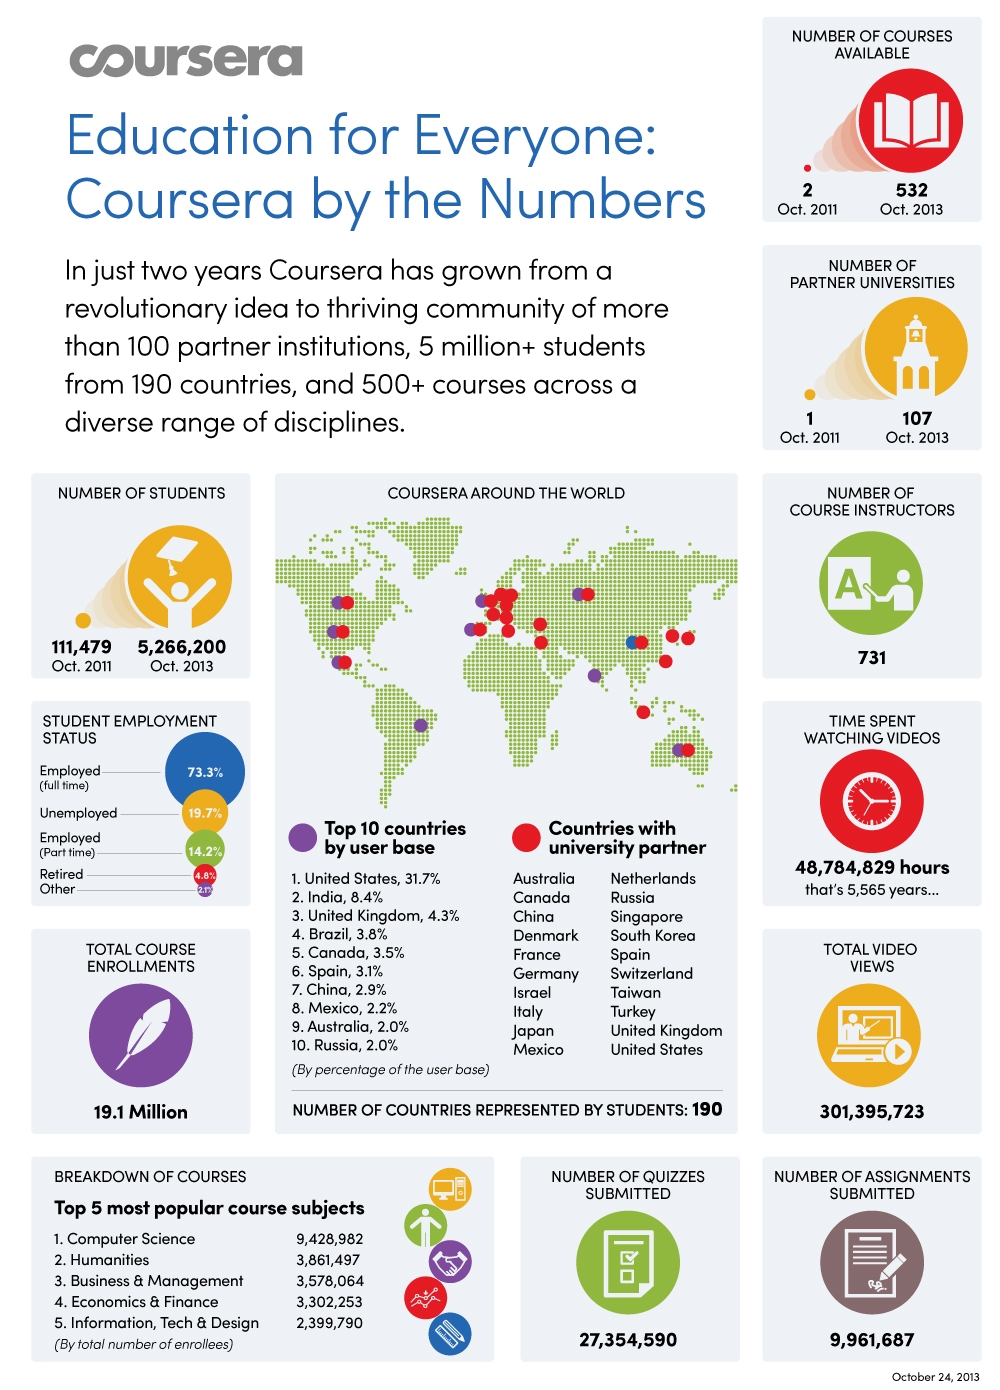
\includegraphics[height=\dimexpr \textheight - 4\baselineskip\relax]{The-Growth-of-Coursera-Infographic}
\caption{The growth of Coursera}
\label{fig:The growth of Coursera}
\end{figure}

One online survey published a "top ten" list of reasons for dropping out.
These were that the course required too much time, or was too difficult or too
basic. Reasons related to poor course design included "lecture fatigue" from
courses that were just lecture videos, lack of a proper introduction to course
technology and format, clunky technology and trolling on discussion boards.
Hidden costs were cited, including required readings from expensive textbooks
written by the instructor that also significantly limited students' access to
learning material. Other non-completers were fiddling around when
they registered, or were participating for knowledge rather than a credential.
Providers are exploring multiple techniques to increase the often single-digit
completion rates in many MOOCs.

As a back side to these impressive figures, which often exceed the
total number of students enrolled in large state universities, has been the massive attrition.
Even if millions of students have registered for courses through Coursera, the
company and its university partners have awarded only 280,000 certificates of
completion.

The rates of completion for students who have given some indication that they
plan to do the work is substantially higher. For example, for students who
submit the first assignment, the completion rate jumps to 45 percent.

For students who are paying \$50 for the company’s new Signature Track
program—which includes features designed as safeguards against identity fraud
and cheating on examinations—the pass rates are even higher, at about 70
percent.

That is even higher than the non-Signature Track students who profess
in surveys to high levels of commitment to completing the course. This suggests
that having skin in the game is highly valuable, and promotes responsibility \citep{courseradropout}.
% idea!

Another issue that might arise with MOOC's, is that of identity fraud and cheating
at exams. This might happen in real life too, but facilitated by large crowd of stundent,
and the ease at which one could be relatively anonymous on the internet, these
two issues could reach a large scale, unfortunately.
% 1 page

\subsection{Towards a better solution}
% tipes of mooc
As MOOCs have evolved, there appear to be two distinct types: those that
emphasize the connectivist philosophy, and those that resemble more traditional
courses. One can distinguish between the two by using the terms "cMOOC" and
"xMOOC", as George Siemens notes it his blog post \citep{moocs_are_a_platform}.
A third type, the "vMOOC", has been suggested to describe
vocational MOOCs, that would require simulations and related technologies to
teach and assess practical skills and abilities.
Such instructional design approaches attempt to connect learners to each other
to answer questions and/or collaborate on joint projects. This may include
emphasizing collaborative development of the MOOC.

One important thing that can help students succeed in an online course is
interpersonal interaction and support says Shanna Smith Jaggars, assistant
director of Columbia University's Community College Research Center. Her
research compared online-only and face-to-face learning in studies of
community-college students and faculty in Virginia and Washington state. Among
her findings: In Virginia, 32\% of students failed or withdrew from for-credit
online courses, compared with 19\% for equivalent in-person courses \citep{early_report_on_moocs}.

Assigning mentors to students is another interaction-enhancing technique.
In 2013 Harvard offered a popular class, The Ancient Greek Hero, taken by
thousands of Harvard students over prior decades. It appealed to alumni to
volunteer as online mentors and discussion group managers. About 10 former
teaching fellows also volunteered. The task of the volunteers, which required
3–5 hours per week, was to focus online class discussion. This edX course registered 27,000 students.
As one student, named Rob, was completing a MOOC  from Stanford U Venture Labs, A crash course in
Creativity by Tina Seelig, where about 22,000 were enrolled, reports a rate of
completion of about 50\% completion on their team of 20. The succes is
attributed to using G+ hangouts, that added an engaging social dimension to adult learning.

Unfortunately, MOOCS still have not yet learned to use the tech tools like
real-time chats effectively. With such collaborative tools, a student can learn
more, and create a more engaging environment, that would not be possible otherwise.

So, beside the issue with cheating, the biggest pain point of these systems is that they are
lacking interactivity: most of them are just a site hosting videos, tasks and a forum for students.
These issues can be addressed technically, by inventing something better.

The project proposed in this thesis, Discite, is taking inspiration from several existing projects, some of which
were mentioned previously, and brings several others features to the table. These projects are:
\begin{enumerate}[topsep=5pt, partopsep=0pt,itemsep=3pt,parsep=1pt]
    \item[--] Coursera;
    \item[--] Prezi;
    \item[--] Iversity;
    \item[--] Udacity;
    \item[--] University of Reddit;
    \item[--] Edx.
\end{enumerate}
Discite doesn't have yet any affiliation program with universities, nor there is a plan
for such an affiliation: the platform is mainly a peer-to-peer one.
Out of the projects that Discite takes inspiration, Prezi is of a special interest, as it has one nice interactive feature: you ca run
a presentation synchronized on several computers. This is a very powerful feature,
that add one extra dimension to e-learning.
% 2 pages
\clearpage
